\section{Publish/Subscribe via a Broker}

\begin{frame}{Publish/Subscribe via a Broker}
      \centering
      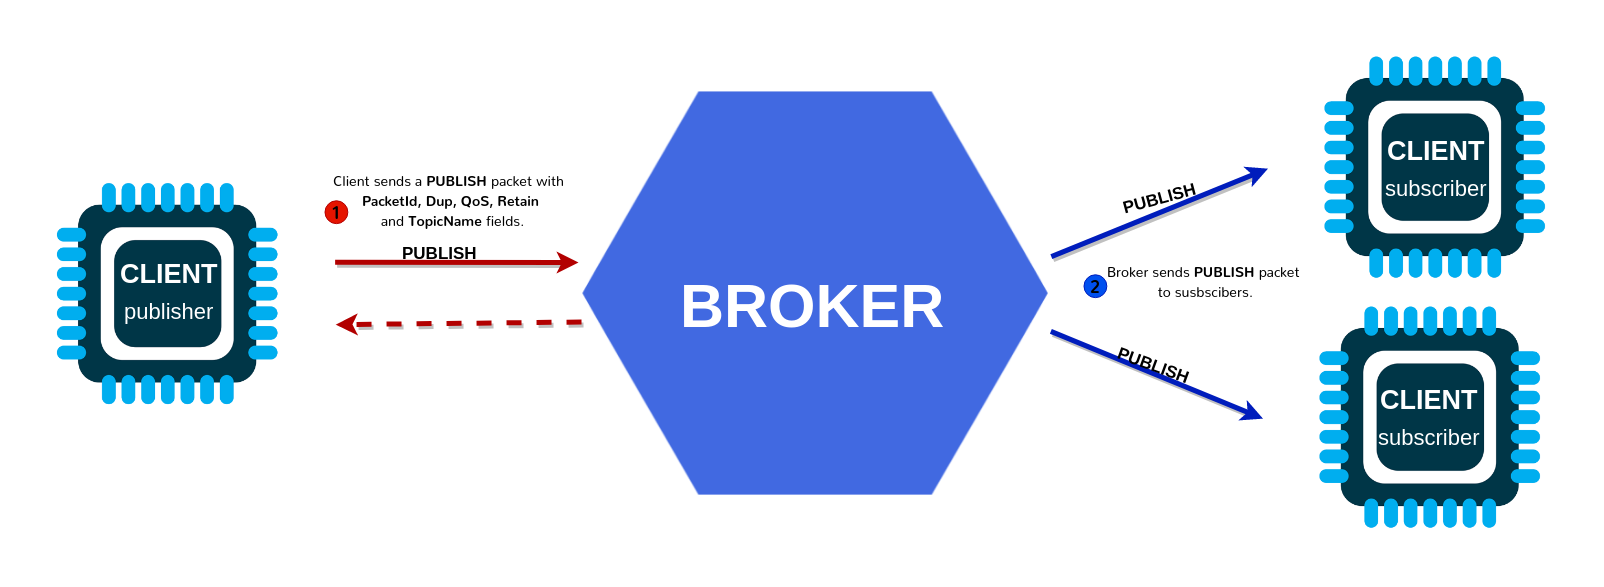
\includegraphics[width=0.9\linewidth]{images/MQTT_publish.png}%

      \begin{itemize}
        \item \textbf{Publish}: send data to a topic (e.g., \texttt{lab/temperature})
        \item \textbf{Subscribe}: receive all messages matching a topic filter
        \item Broker \textbf{routes} messages to all matching subscribers (many-to-many)
        \item No need for publishers to know who is listening
      \end{itemize}

\end{frame}
